\documentclass[10pt]{article}

\usepackage[margin=0.78in]{geometry}
\usepackage[T1]{fontenc}
\usepackage{lmodern}
\usepackage{microtype}
\usepackage{amsmath,amssymb,bm}
\usepackage{booktabs}
\usepackage{graphicx}
\usepackage{xcolor}
\usepackage{hyperref}
\usepackage{enumitem}

\hypersetup{colorlinks=true,linkcolor=blue!55!black,urlcolor=blue!55!black}
\setlist{nosep,leftmargin=1.4em}
\newcommand{\bfr}{\boldsymbol r}
\newcommand{\hc}{\hat c}
\newcommand{\hr}{\hat r}
\newcommand{\Tr}{\operatorname{Tr}}
\newcommand{\tr}{\operatorname{tr}}

\title{CPU pilot for spacetime anisotropy from Gaussian reference ancillas}
\author{Numerical methods and pilot report}
\date{August 26, 2026}

\begin{document}
\maketitle

\begin{abstract}
We implement the reference-qubit spacetime-correlation protocol of Zabalo
\emph{et al.} in the charge-conserving Gaussian adaptive circuit.  A wall unit
cell and a two-mode spectator reference are prepared in a maximally entangled
Gaussian state, the canonical adaptive circuit continues, and the exact mutual
information between two reference subsystems is evaluated from their reduced
correlation matrix.  The implementation passes analytic Bell-pair tests and a
canonical-engine integration test.  A CPU pilot at circumferences $L=6,8$ with
four Born trajectories per configuration shows that the observable is feasible
and has a long-lived signal.  It does not yet calibrate the anisotropy: the
distribution is rare-event dominated, the $L=6$ crossing is only a candidate,
and the $L=8$ mean curve is nonmonotone because of one large trajectory.  The
pilot supports a next run with at least $S=100$ trajectories per configuration
and roughly $7L$ total cycles per anisotropy trajectory.
\end{abstract}

\section{Conclusion first}

\paragraph{Protocol correction.}
The completed run documented below used an explicit domain wall with
\path{dw_truncation=False} and \path{meas_slab_only=False}.  The target
campaign is now locked to \path{dw_truncation=True} and
\path{meas_slab_only=True}.  The saved run remains a valid engineering
test of Gaussian reference insertion, entropy evaluation, and statistical
failure modes, but its candidate $\alpha$ is not a calibration of the
support-terminated protocol.  The target geometry requires a new convergence
and anisotropy run; no result below is silently relabeled.

The correct reference observable can be implemented without leaving the
Gaussian covariance/occupied-frame description.  The pilot therefore resolves
the earlier engineering question: reference ancillas are not blocked by the
noninvertibility of individual measurement maps or by nonfinite many-body log
singular values.  They are ordinary spectator fermionic modes carried by the
pure Gaussian frame.

The present numerical result is a \emph{feasibility success} but not an accepted
measurement of $\alpha$.  The strict analysis gives
\begin{align*}
L=6:&\quad t_*=1.448,\qquad \alpha_{\rm cand}=1.163,
\\
L=8:&\quad t_*\text{ unresolved}.
\end{align*}
For $L=6$, only $75.6\%$ of trajectory-bootstrap resamples contain a valid
ordered crossing, and the earlier permissive 95\% interval was broad.  For
$L=8$, the temporal mean begins below the spatial target, rises at the second
separation because of a single rare trajectory, and then falls.  A late
downward interpolation through that upward fluctuation is not a CFT matching
point and is rejected.

\section{CFT matching prescription}

For a primary field of scaling dimension $\Delta$ on a cylinder of spatial
circumference $L$, an anisotropic Euclidean coordinate is
$z'=\alpha t+iy$.  The plane-to-cylinder map gives the equal-time,
half-circumference correlator and the equal-position temporal correlator as
\begin{align}
g_{\rm space}'(L/2,0)
  &=\left(\frac{\pi}{L}\right)^{2\Delta},
\\
g_{\rm time}'(0,t)
  &=\left(\frac{\pi}{L}\right)^{2\Delta}
    \left[\sinh\left(\frac{\pi\alpha t}{L}\right)\right]^{-2\Delta}.
\end{align}
At the matching time $t_*$, the unknown scaling dimension cancels:
\begin{equation}
g_{\rm time}'(0,t_*)=g_{\rm space}'(L/2,0)
\quad\Longrightarrow\quad
\boxed{\alpha=\frac{\ln(1+\sqrt 2)L}{\pi t_*}}.
\label{eq:alpha}
\end{equation}
This is the prescription in the supplemental ``Anisotropy parameter'' section
of Zabalo \emph{et al.}, Phys. Rev. Lett. \textbf{128}, 050602 (2022),
\href{https://arxiv.org/abs/2107.03393}{arXiv:2107.03393}.

The numerical proxy for $g'$ is the mutual information between two reference
systems that were locally entangled with the circuit at the two spacetime
points.  The spatial insertion uses $(\delta y,\delta\tau)=(L/2,0)$; the
temporal insertion uses $(0,\delta\tau)$.  The same definition of the reference
observable must be used on both legs of the match.

\section{Charge-conserving Gaussian reference construction}

\subsection{Conventions}

Let $P$ denote the physical system and $R$ a spectator reference.  For complex
fermions $\hat\psi_i$, use the project correlation matrix
\begin{equation}
G_{ij}=\Tr(\hat\rho\,\hat\psi_i^\dagger\hat\psi_j).
\end{equation}
A pure, charge-conserving Gaussian state is stored as an orthonormal occupied
frame $F$.  With the row convention used by the code,
$G=F^*F^{\mathsf T}$, while the transposed one-body matrix materialized by the
frame is $FF^\dagger$; the two have identical subsystem spectra.  The circuit
has two canonical physical modes $\hc_{\bfr,\mu}$, $\mu=0,1$, per unit cell.

\subsection{One physical mode and one reference mode}

For a normalized physical mode $\hat f$, first measure
$\hat f^\dagger\hat f$ with Born probability $p=\langle\hat f^\dagger\hat
f\rangle$, obtaining $m\in\{0,1\}$.  Measurement factorizes this mode from the
remaining system.  Append a reference mode $\hr$ in the complementary
occupation $1-m$ and apply a 50:50 number-conserving beam splitter,
\begin{equation}
\begin{pmatrix}\hat f'\\ \hr'\end{pmatrix}
=\frac{1}{\sqrt2}
\begin{pmatrix}1&1\\-1&1\end{pmatrix}
\begin{pmatrix}\hat f\\ \hr\end{pmatrix}.
\label{eq:beam-splitter}
\end{equation}
Before Eq.~\eqref{eq:beam-splitter}, the pair contains exactly one fermion.
After it, the pair is a one-particle Bell state, up to an outcome-dependent
phase.  Its correlation matrix has diagonal entries $1/2$ and eigenvalues
$0,1$; the reference occupation is $1/2$ and $S(R)=\ln2$.  Thus both possible
measurement outcomes yield the same amount of entanglement, no outcome is
postselected, Gaussianity is preserved, and total charge on $P\cup R$ is
conserved.

\subsection{A full wall unit cell}

The local Hilbert space of one unit cell contains two fermion modes and has
dimension four.  We apply the construction independently to $\mu=0,1$.
Consequently each reference subsystem contains two modes, the freshly inserted
cell/reference state is maximally entangled across this four-level cut, and
\begin{equation}
S(R_{\rm fresh})=2\ln2.
\end{equation}
Using both canonical modes avoids choosing one orbital flavor as a
post-hoc definition of the local operator.

\subsection{Reference mutual information}

If $A$ is any collection of reference rows, the code forms the transposed
reduced correlation matrix $\widetilde G_A=F_AF_A^\dagger$.  If $n_k$ are its
eigenvalues (equivalently those of $G_A$), then
\begin{equation}
S(A)=-\sum_k\left[n_k\ln n_k+(1-n_k)\ln(1-n_k)\right].
\end{equation}
The measured correlator is
\begin{equation}
I(R_1:R_2)=S(R_1)+S(R_2)-S(R_1R_2).
\label{eq:mi}
\end{equation}
Only $2\times2$ and $4\times4$ reduced correlation matrices are diagonalized.
No full covariance history or Fock-space density matrix is required.

\section{Circuit protocol and implementation}

For every independent trajectory and every probe configuration:
\begin{enumerate}
\item Run the canonical CPU dynamics to $\tau_1=4L$.
\item At one programmed wall and a uniformly sampled $y_1$, insert $R_1$ using
      the two-mode construction above.
\item Insert $R_2$ either at $(y_1+L/2,\tau_1)$ for the spatial correlator or at
      $(y_1,\tau_1+\delta\tau)$ for the temporal correlator.
\item Continue the same Born trajectory for $2L$ additional cycles after the
      second insertion.  Save $I(R_1:R_2)$, $S(R_1)$, $S(R_2)$, and $S(R_1R_2)$
      at relative follow cycles $u=0,1,\ldots,2L$.
\item Define the pilot plateau estimator as the average over $u=L+1,\ldots,2L$.
\end{enumerate}

The model is the current explicit-interface production geometry:
\begin{center}
\begin{tabular}{ll}
\toprule
Quantity & Pilot setting\\
\midrule
Transverse size & $N_x=20$\\
Wall circumference & $L=N_y=6,8$\\
Walls & canonical \texttt{DW\_loc} $=(4,16)$\\
OW range & $n_{\rm shell}=1$\\
Mass parameters & $\alpha_1=1$, $\alpha_2=30$\\
Schedule & random permutation per cycle\\
Feedback & perfect correction\\
Initialization & default pure physical frame\\
Samples & $S=4$ per spatial/temporal configuration\\
Temporal grid & $\delta\tau=1,\ldots,5$ for $L=6$; $1,\ldots,6$ for $L=8$\\
\bottomrule
\end{tabular}
\end{center}

Every trajectory calls
\texttt{classA\_U1FGTN.run\_markov\_circuit(...)}.  The pilot extends the live
occupied frame by four spectator rows through the native-cycle observer.  All
subsequent overcomplete-Wannier measurements act only on the original
$2N_xN_y$ system rows; correlations with the spectator rows nevertheless
update automatically through the occupied frame.  The final dimension is
$2N_xN_y+4$.

This live-state insertion is deliberately isolated in the CPU pilot.  Before a
production campaign, it should become an explicit reference-insertion hook in
the canonical engine, with the same algebra and tests, rather than remain an
observer side effect.

\section{Validation}

Five focused tests pass.
\begin{itemize}
\item Empty and occupied input modes both produce a Bell pair with pair
      correlation eigenvalues $0,1$, occupations $1/2,1/2$, and reference
      entropy $\ln2$.
\item Two freshly and independently inserted two-mode references have
      $I(R_1:R_2)=0$, while $S(R_1)=S(R_2)=2\ln2$ and
      $S(R_1R_2)=4\ln2$.
\item Linear matching recovers a known synthetic $t_*$ and Eq.~\eqref{eq:alpha}.
\item A nonphysical upward noise excursion cannot create a late crossing.
\item The canonical engine continues after all four spectator modes are added;
      the augmented frame remains orthonormal and all reference observables are
      finite and nonnegative.
\end{itemize}
The separate end-to-end smoke run and the production-size pilot both completed
without missing cycles.  The augmented-frame Gram residual remained below the
hard $10^{-8}$ check (the direct integration smoke gave approximately
$10^{-15}$).

\section{Estimator and statistical rules}

The two walls are balanced across sample indices, but they are not promoted to
independent samples.  A complete Born trajectory is the statistical unit.
Spatial and temporal configurations use matched sample/seed identities, and
the nonparametric bootstrap resamples these identities jointly.

The mean temporal curve must begin above the spatial target and cross it
downward as $\delta\tau$ increases.  If the shortest sampled temporal point is
already below the target, a later upward fluctuation followed by a downward
fluctuation is rejected.  Within a valid adjacent bracket, $t_*$ is found by
linear interpolation and inserted in Eq.~\eqref{eq:alpha}.  This rule is more
restrictive than merely finding any sign change, and prevents rare-trajectory
noise from manufacturing an anisotropy.

\section{Pilot results}

\begin{figure}[t]
\centering
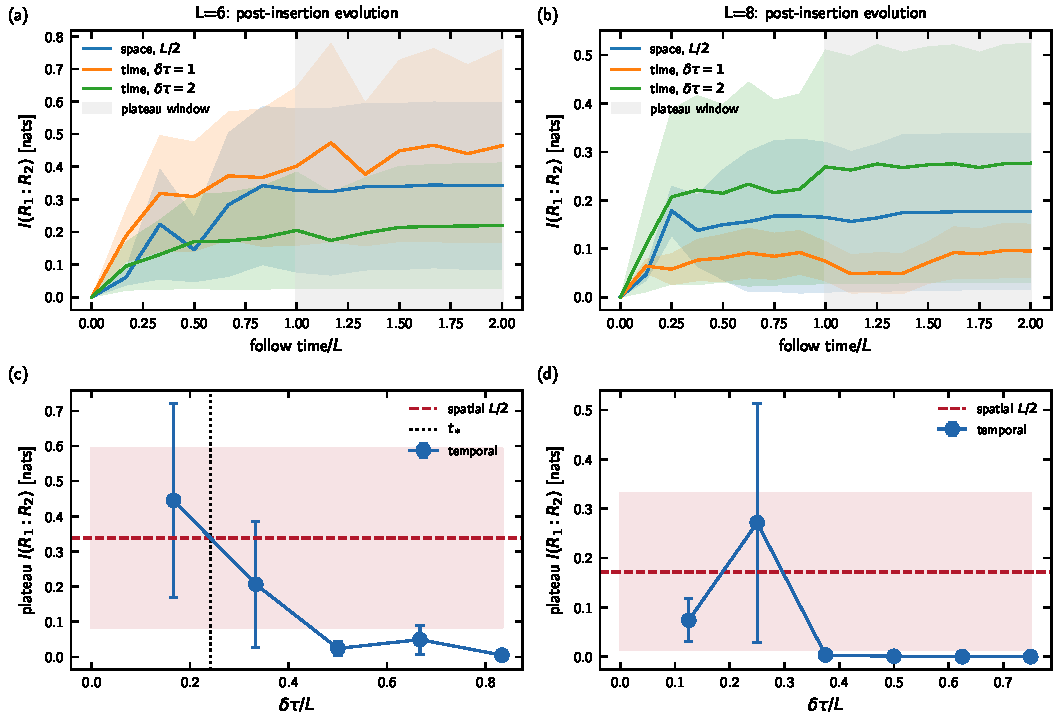
\includegraphics[width=\textwidth]{../outputs/pilot_20260826_183458/reference_anisotropy_pilot.pdf}
\caption{Reference-ancilla CPU pilot.  Top: post-insertion mutual-information
evolution; shading is the trajectory standard error and gray marks the final
$L$-cycle plateau window.  Bottom: plateau temporal correlators and the spatial
$L/2$ target.  For $L=6$ the mean has an ordered candidate crossing between
$\delta\tau=1,2$.  For $L=8$ the large $\delta\tau=2$ point is supplied mainly
by one trajectory; because the $\delta\tau=1$ mean is already below the spatial
target, the strict analysis rejects the apparent later crossing.}
\label{fig:pilot}
\end{figure}

\begin{table}[t]
\centering
\caption{Strict matching results.  Bootstrap resolution is the fraction of
whole-trajectory resamples that contain an ordered downward bracket.}
\begin{tabular}{cccccc}
\toprule
$L$ & $\overline I_{\rm space}$ & $t_*$ & $\alpha$ & bootstrap resolution & estimated $S$ for 20\% spatial SEM\\
\midrule
6 & 0.3383 & 1.448 & 1.163 (candidate) & 0.756 & 57\\
8 & 0.1721 & unresolved & unresolved & 0.266 & 85\\
\bottomrule
\end{tabular}
\label{tab:results}
\end{table}

The temporal plateau means are
\begin{align*}
L=6:&\quad (0.4450,\ 0.2067,\ 0.0241,\ 0.0492,\ 0.00492),\\
L=8:&\quad (0.0741,\ 0.2719,\ 0.00350,\ 0.00104,\ 7.54\!\times\!10^{-5},\ 8.03\!\times\!10^{-5}).
\end{align*}
The $L=8$ ordering violation is visible directly: the second point is larger
than the first.  At the trajectory level, one of four samples contributes
$0.9973$ to the $\delta\tau=2$ plateau, while the other three contribute
$2.9\times10^{-6}$, $8.8\times10^{-3}$, and $8.15\times10^{-2}$.  Likewise,
one trajectory contributes $0.6458$ of the $L=8$ spatial signal while two are
near $10^{-6}$.  This is the broad, rare-event-dominated distribution expected
for reference mutual information in monitored dynamics; a four-sample mean is
not stable.

The plateau diagnostic compares the preceding and final $L$-cycle windows.
For the configurations that control the candidate bracket, the paired changes
are
\begin{center}
\begin{tabular}{lcc}
\toprule
Configuration & previous $L$-window & final $L$-window; paired change\\
\midrule
$L=6$, spatial & 0.2305 & 0.3383; $+0.1078\pm0.0977$\\
$L=6$, $\delta\tau=1$ & 0.3258 & 0.4450; $+0.1192\pm0.1045$\\
$L=6$, $\delta\tau=2$ & 0.1595 & 0.2067; $+0.0472\pm0.0448$\\
$L=8$, spatial & 0.1461 & 0.1721; $+0.0260\pm0.0602$\\
$L=8$, $\delta\tau=1$ & 0.0778 & 0.0741; $-0.0037\pm0.0188$\\
$L=8$, $\delta\tau=2$ & 0.2117 & 0.2719; $+0.0602\pm0.0557$\\
\bottomrule
\end{tabular}
\end{center}
Errors here are standard errors of the four paired trajectory changes.  The
$L=6$ controlling curves still rise by roughly one standard error, reinforcing
the decision to call its crossing a candidate rather than a calibration.

\section{Why the earlier record-field pilot failed}

Before implementing references, a surrogate pilot compared connected local
record surprisal and mismatch activity in space and time.  Those observables
had a large lag-zero contact term and noise-scale correlations at every nonzero
lag and at $L/2$.  Interpolating from lag zero to lag one produced fictitious
sub-cycle crossings.  Once the contact term was excluded, all cases were
unresolved.  This was an estimator mismatch, not evidence that the wall lacks
an anisotropic critical sector.  The present reference pilot confirms the
distinction: it produces a nonzero, evolving, long-lived mutual-information
signal.

\section{Recommended next CPU campaign}

\subsection{How the necessary cycle count is determined}

The three contributions to trajectory length answer different questions and
must not be conflated:
\begin{equation}
T_{\rm total}=T_{\rm eq}+\delta\tau_{\max}+T_{\rm follow}.
\label{eq:cycle-budget}
\end{equation}
$T_{\rm eq}$ removes dependence on the initial Gaussian state;
$\delta\tau_{\max}$ is only the temporal distance needed to bracket $t_*$; and
$T_{\rm follow}$ allows the two-reference mutual information to reach its
late-time value after the second insertion.

For the support-terminated geometry, determine these terms with matched Born
seeds as follows.
\begin{enumerate}
\item Run an equilibration grid $T_{\rm eq}/L=2,3,4,6$ while holding a long
      $T_{\rm follow}=3L$.  For the spatial point and the two temporal points
      bracketing the crossing, compare adjacent equilibration choices using the
      paired trajectory differences.  Accept the smallest $T_{\rm eq}$ for
      which the 95\% paired-bootstrap interval contains zero, the point shift is
      smaller than half the final standard error, and the inferred $t_*/L$ is
      stable under the next larger choice.
\item In a run followed through at least $3L$, form consecutive nonoverlapping
      $L$-cycle window means after the second insertion.  Accept the smallest
      $T_{\rm follow}$ for which the last two windows pass the same paired
      zero-shift and half-standard-error criteria for the spatial point and both
      bracketing temporal points.  If no pair passes, extend the follow to $4L$
      rather than broadening the averaging window until drift is hidden.
\item Increase $\delta\tau$ only until the mean temporal correlator has an
      ordered downward bracket around the spatial target.  Once a preliminary
      anisotropy is available, the expected location is
      \begin{equation}
      \frac{t_*}{L}=\frac{\ln(1+\sqrt2)}{\pi\alpha}
      \simeq\frac{0.28055}{\alpha}.
      \end{equation}
      Add every integer cycle inside that bracket; points far beyond it do not
      improve the interpolation.
\end{enumerate}
The audit must be performed on the same support-terminated protocol and cycle
definition as production.  Copying Zabalo's $4L$ equilibration from a different
circuit, or copying the untruncated pilot, does not establish convergence.

The sample coefficient of variation is $1.51$ ($L=6$ spatial) and $1.84$
($L=8$ spatial).  The elementary estimate
\begin{equation}
S_{20\%}\simeq\left(\frac{\mathrm{CV}}{0.20}\right)^2
\end{equation}
gives 57 and 85 trajectories merely to reach a 20\% relative standard error on
the spatial mean.  Temporal configurations in the scanned range require
approximately 31--100 trajectories by the same diagnostic.  Therefore:
\begin{enumerate}
\item use at least $S=100$ trajectories per configuration for the next
      calibration pilot; $S=200$ is preferable before quoting a production
      uncertainty;
\item retain $L=6,8$ and add $L=10$ only after the first two sizes show a stable
      ordered bracket;
\item keep $\tau_1=4L$ and a $2L$ post-insertion follow initially, but require
      agreement between the preceding and final $L$ windows; extend to $3L$ if
      that test fails;
\item use a coarse temporal grid through $0.75L$, then add every integer cycle
      only inside the resolved bracket;
\item report the arithmetic Born mean and the full trajectory distribution;
      do not replace the mean by a typical or median mutual information.
\end{enumerate}

For the present protocol, the largest trajectory length is
\begin{equation}
T_{\rm aniso}=4L+0.75L+2L=6.75L,
\end{equation}
so allocating $7L$ cycles per reference-anisotropy trajectory is appropriate.
This is the initial cycle budget for the \emph{calibration experiment}, not an
assumed necessary duration and not yet a measured conversion factor for every
other production observable.  It must be checked anew with
\texttt{dw\_truncation=meas\_slab\_only=True}.  Once
$\alpha$ is stable, the natural CFT time unit is $L/\alpha$ and production
aspect ratios can be stated as $\alpha T/L$.

The completed 52-trajectory-configuration pilot used 455.9 CPU seconds.  At the
observed serial rate, $S=100$ over the same $L=6,8$ grid is about 3.2 CPU-hours
and is straightforward to distribute across independent worker processes.

\section{Artifacts and reproducibility}

The implementation and outputs are contained in
\path{00_WORKSPACE/CURRENT/reference_ancilla_anisotropy_cpu_pilot}.
The key files are:
\begin{itemize}
\item \texttt{reference\_probe.py}: Gaussian insertion, entropies, mutual
      information, and strict matching;
\item \texttt{run\_cpu\_pilot.py}: canonical dynamics runner, raw retention,
      bootstrap, and figures;
\item \texttt{reanalyze\_output.py}: lossless strict reanalysis of a completed
      run;
\item \texttt{tests/}: analytic and canonical integration tests;
\item \texttt{outputs/pilot\_20260826\_183458/}: manifest, complete raw NPZ
      arrays, bootstrap arrays, JSON results, summary, and figure.
\end{itemize}
Each raw configuration file retains, with logical leading axes
$(\text{sample},\text{follow cycle})$, the mutual information and all three
component entropies.  It also stores both insertion sites, both orbital
outcomes and Born probabilities, engine and probe seeds, absolute cycle
coordinates, and the canonical dynamics entry point.  The manifest records
source hashes and the dirty Git state.  The superseded permissive interpolation
is preserved as a diagnostic and is not silently overwritten as an accepted
result.

Reproduce the validation and run with
\begin{verbatim}
pytest -q 00_WORKSPACE/CURRENT/reference_ancilla_anisotropy_cpu_pilot/tests
python 00_WORKSPACE/CURRENT/reference_ancilla_anisotropy_cpu_pilot/run_cpu_pilot.py
\end{verbatim}

\end{document}
